\begin{figure}[t]
  \centering
  \begin{subfigure}[b]{.3\linewidth}
    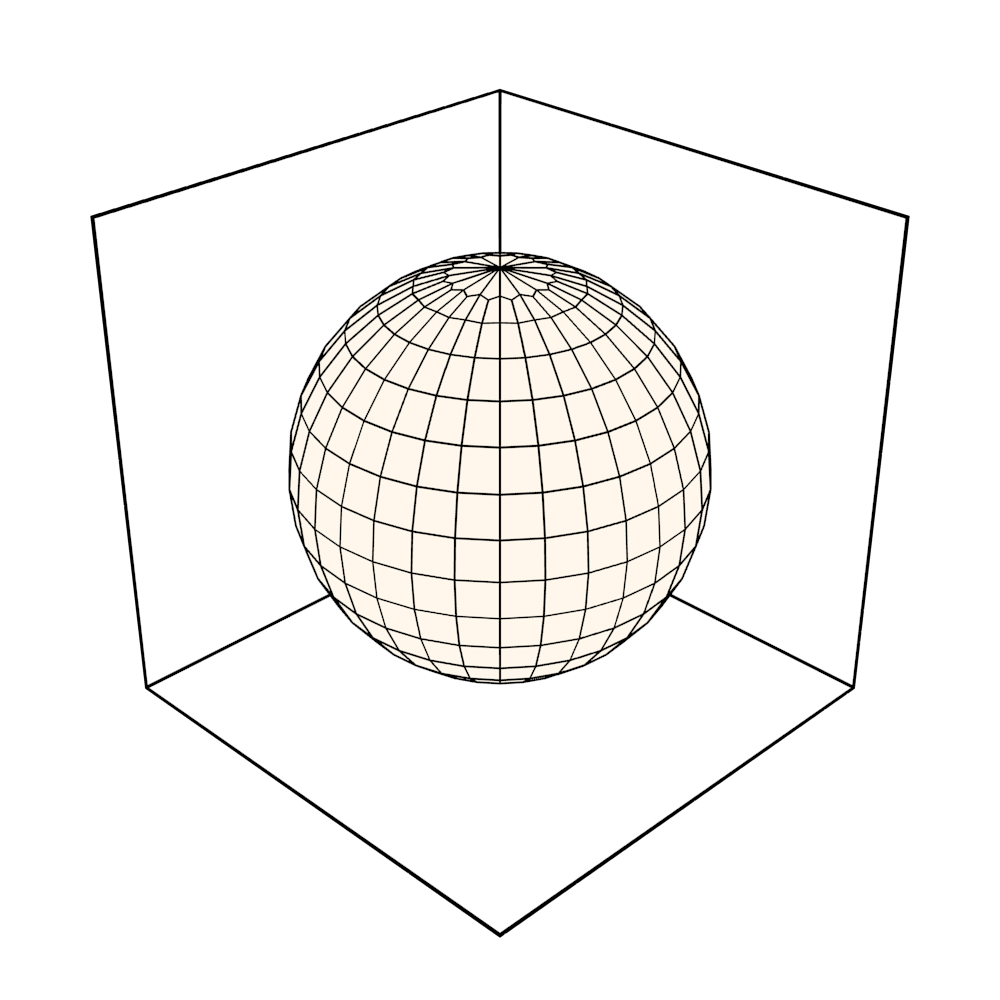
\includegraphics[width=\textwidth]{./img/raw/hs-slt-algorithm/hs-slt-algorithm-1.png}%
    \caption{\footnotesize Initial light volume}%
    \label{fig:hs-p1a}%
  \end{subfigure}
  %
  \begin{subfigure}[b]{.3\linewidth}
    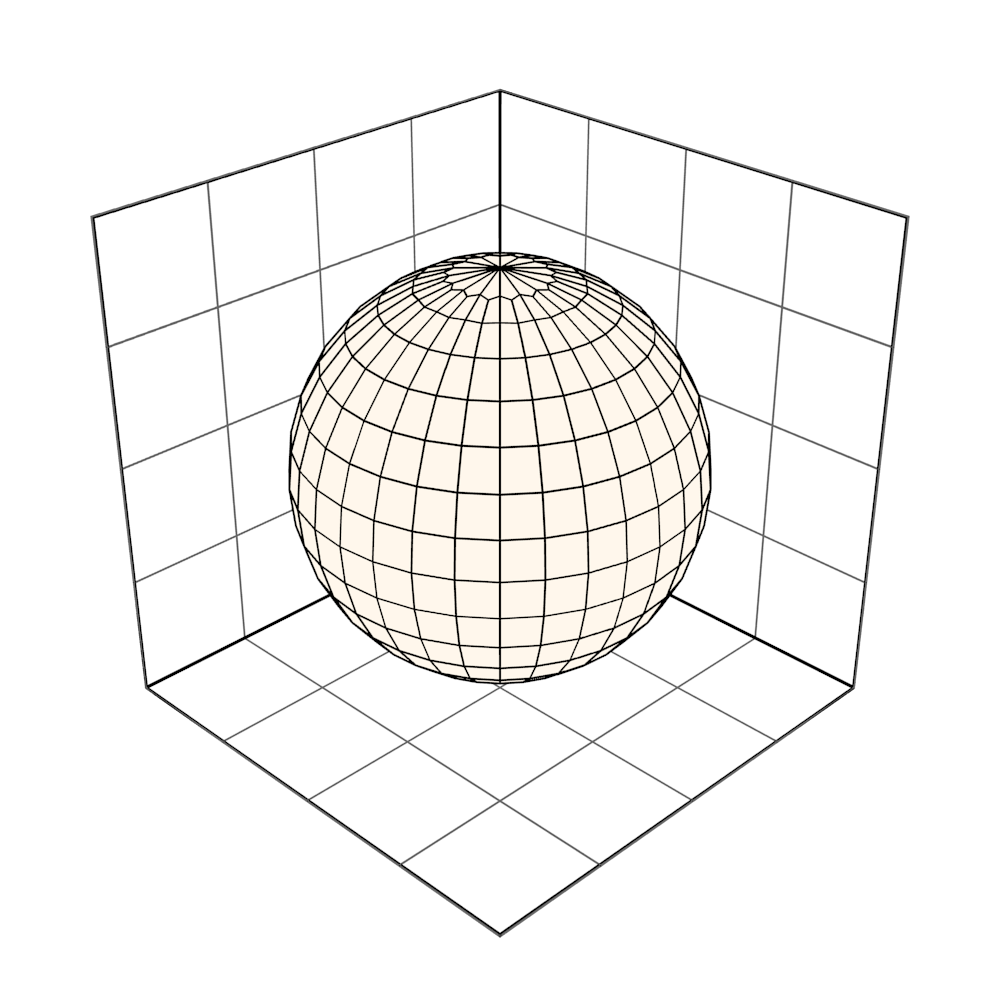
\includegraphics[width=\textwidth]{./img/raw/hs-slt-algorithm/hs-slt-algorithm-2.png}%
    \caption{\footnotesize Define grid}%
    \label{fig:hs-p1b}%
  \end{subfigure}
  %
  \begin{subfigure}[b]{.3\linewidth}
    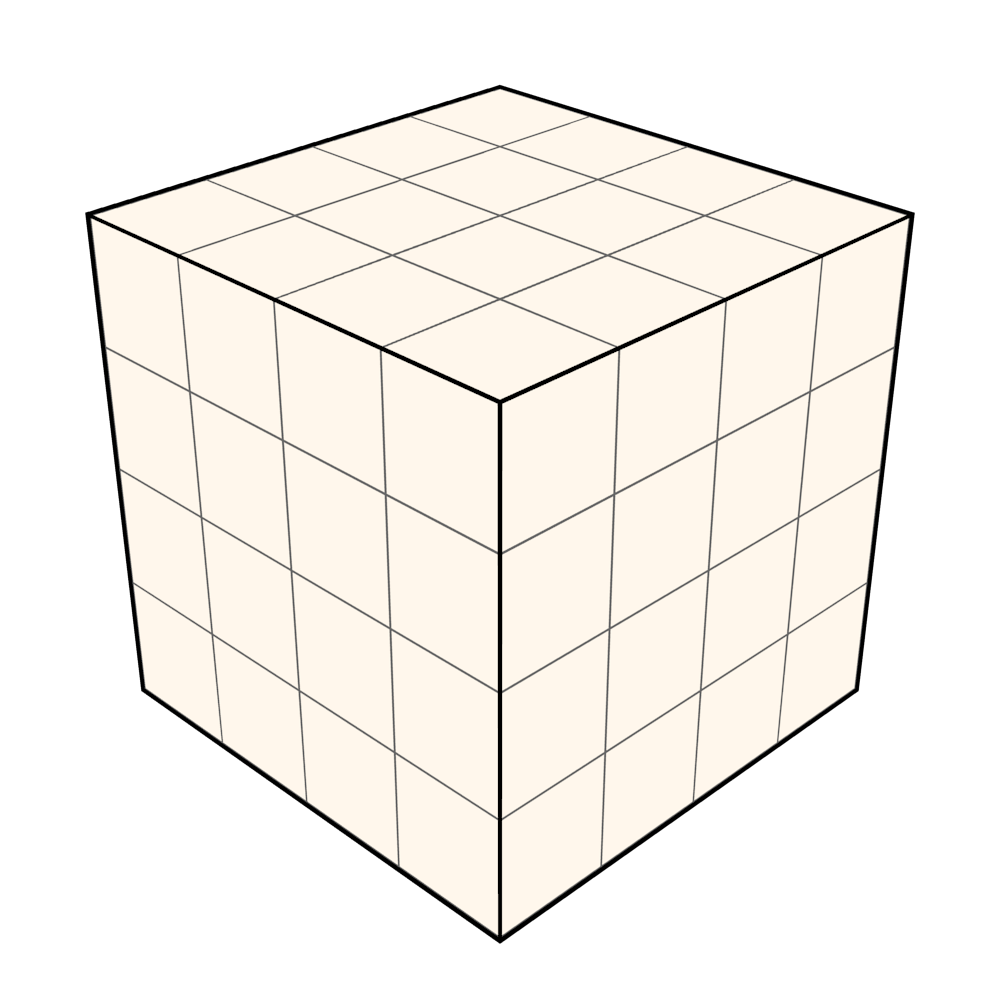
\includegraphics[width=\textwidth]{./img/raw/hs-slt-algorithm/hs-slt-algorithm-3.png}%
    \caption{\footnotesize Initialise grid}%
    \label{fig:hs-p1c}%
  \end{subfigure}
  \\
  \begin{subfigure}[b]{.3\linewidth}
    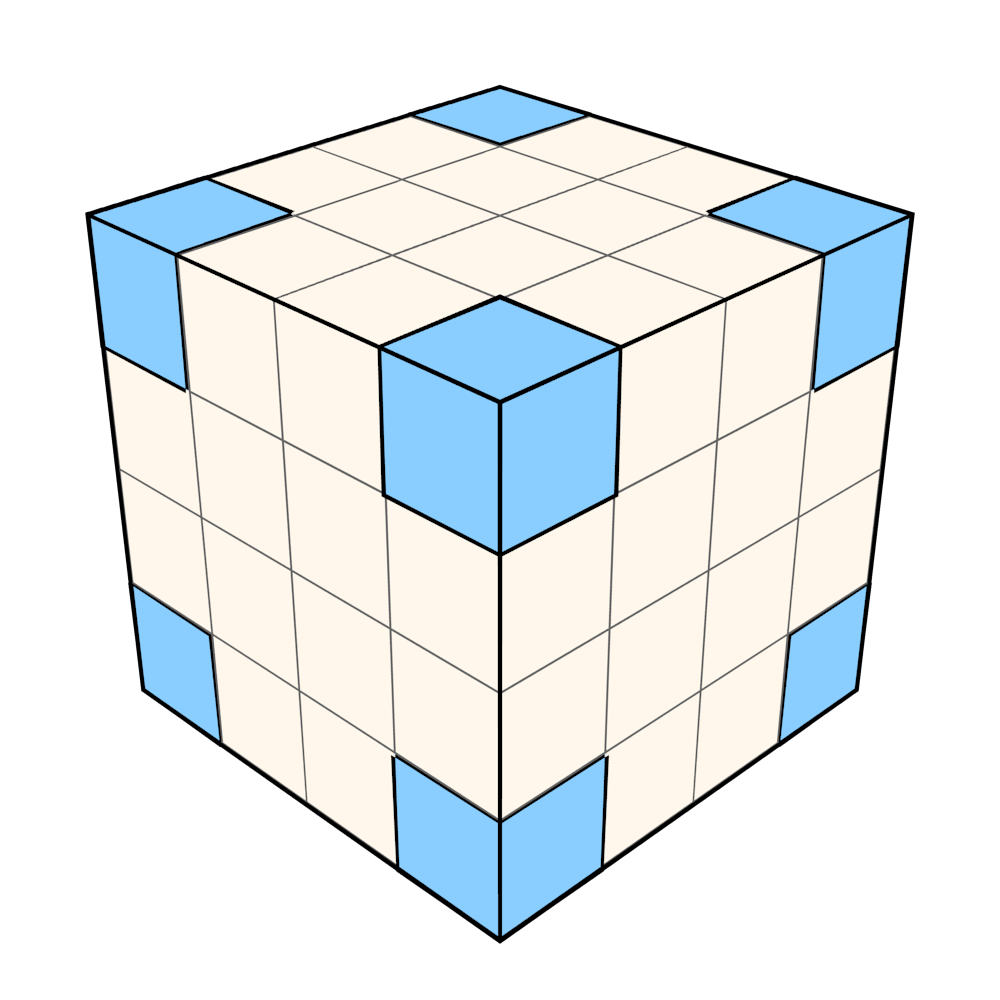
\includegraphics[width=\textwidth]{./img/raw/hs-slt-algorithm/hs-slt-algorithm-4.png}%
    \caption{\footnotesize Evaluate nodes}%
    \label{fig:hs-p1d}%
  \end{subfigure}
  %
  \begin{subfigure}[b]{.3\linewidth}
    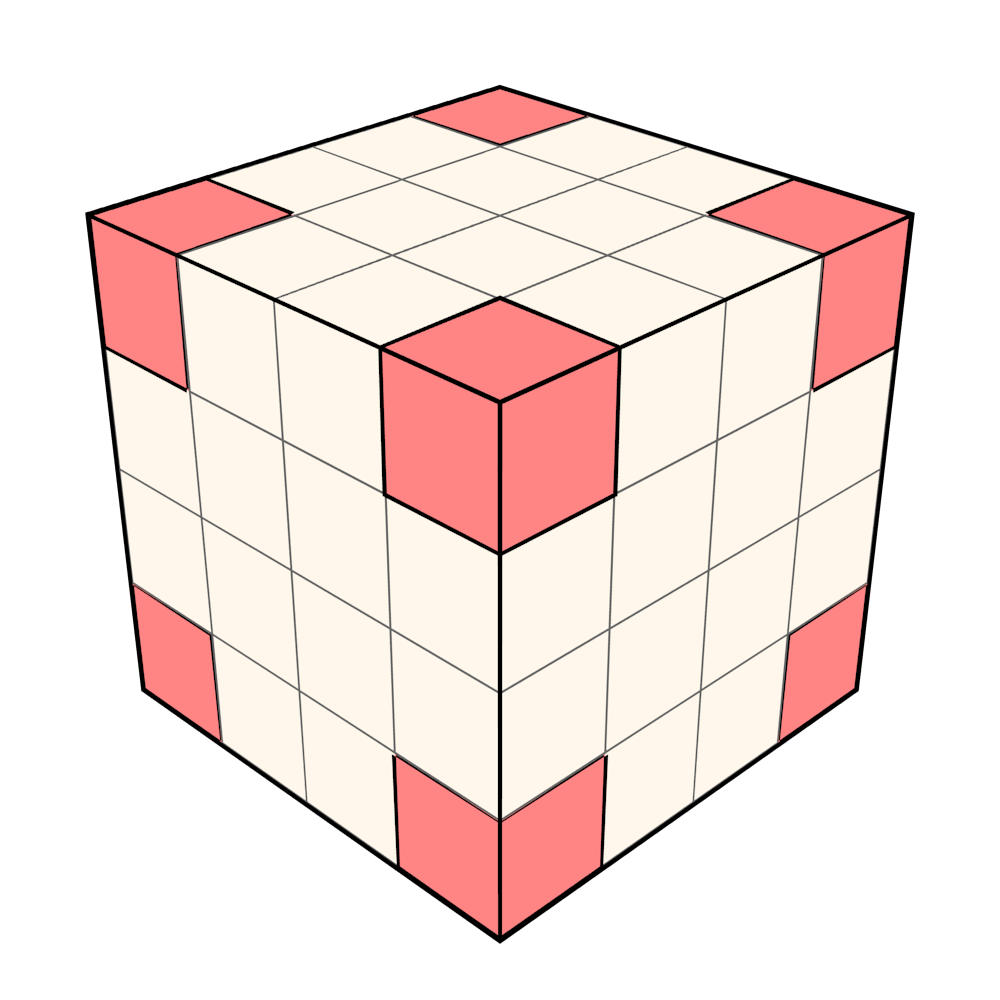
\includegraphics[width=\textwidth]{./img/raw/hs-slt-algorithm/hs-slt-algorithm-5.png}%
    \caption{\footnotesize Mark nodes}%
    \label{fig:hs-p1e}%
  \end{subfigure}
  %
  \begin{subfigure}[b]{.3\linewidth}
    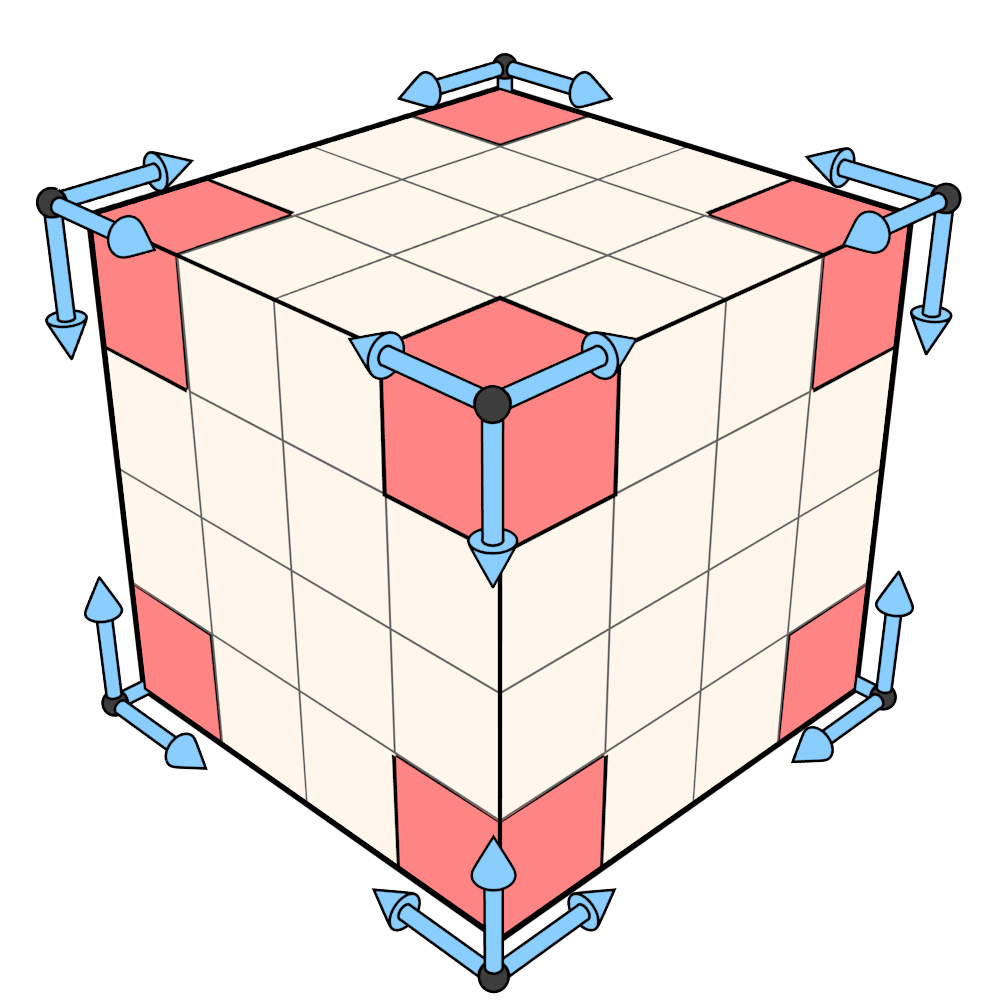
\includegraphics[width=\textwidth]{./img/raw/hs-slt-algorithm/hs-slt-algorithm-6.png}%
    \caption{\footnotesize Select nodes}%
    \label{fig:hs-p1f}%
  \end{subfigure}
  \\
  \begin{subfigure}[b]{.3\linewidth}
    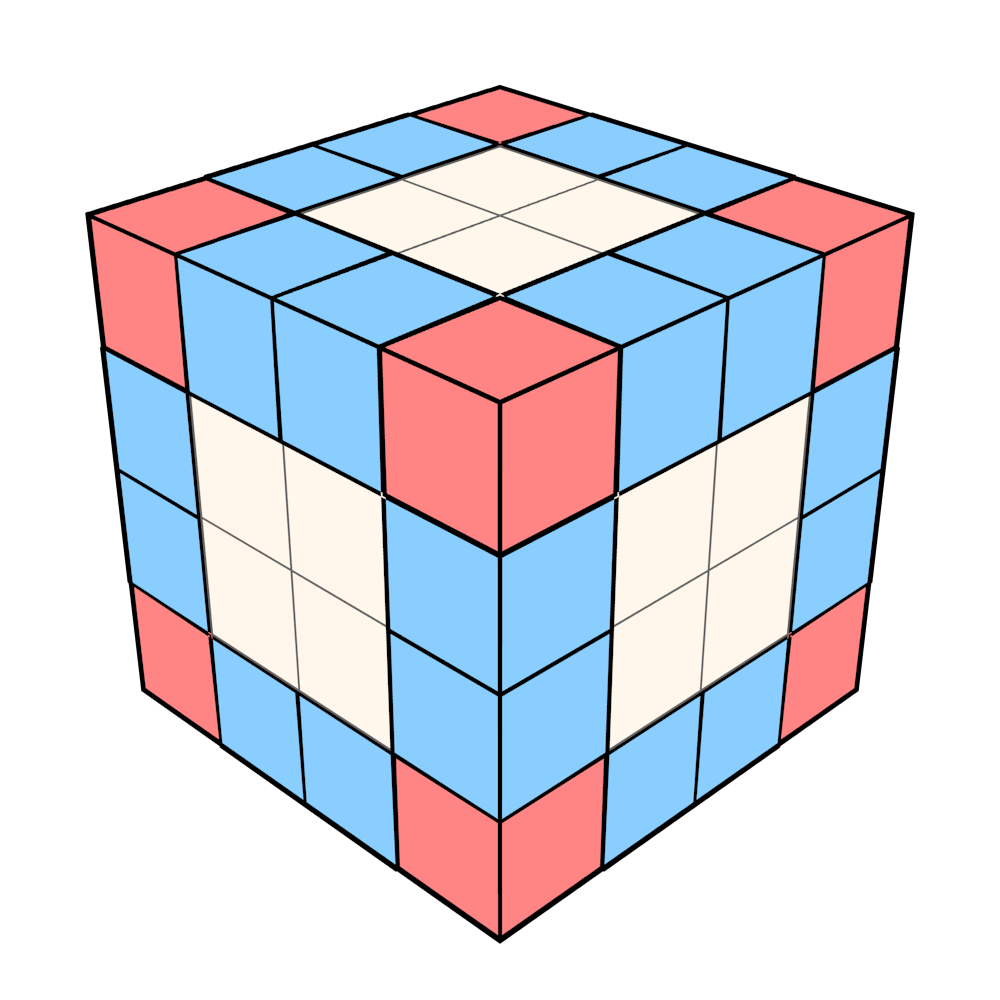
\includegraphics[width=\textwidth]{./img/raw/hs-slt-algorithm/hs-slt-algorithm-7.png}%
    \caption{\footnotesize Evaluate nodes}%
    \label{fig:hs-p1g}%
  \end{subfigure}
  %
  \begin{subfigure}[b]{.3\linewidth}
    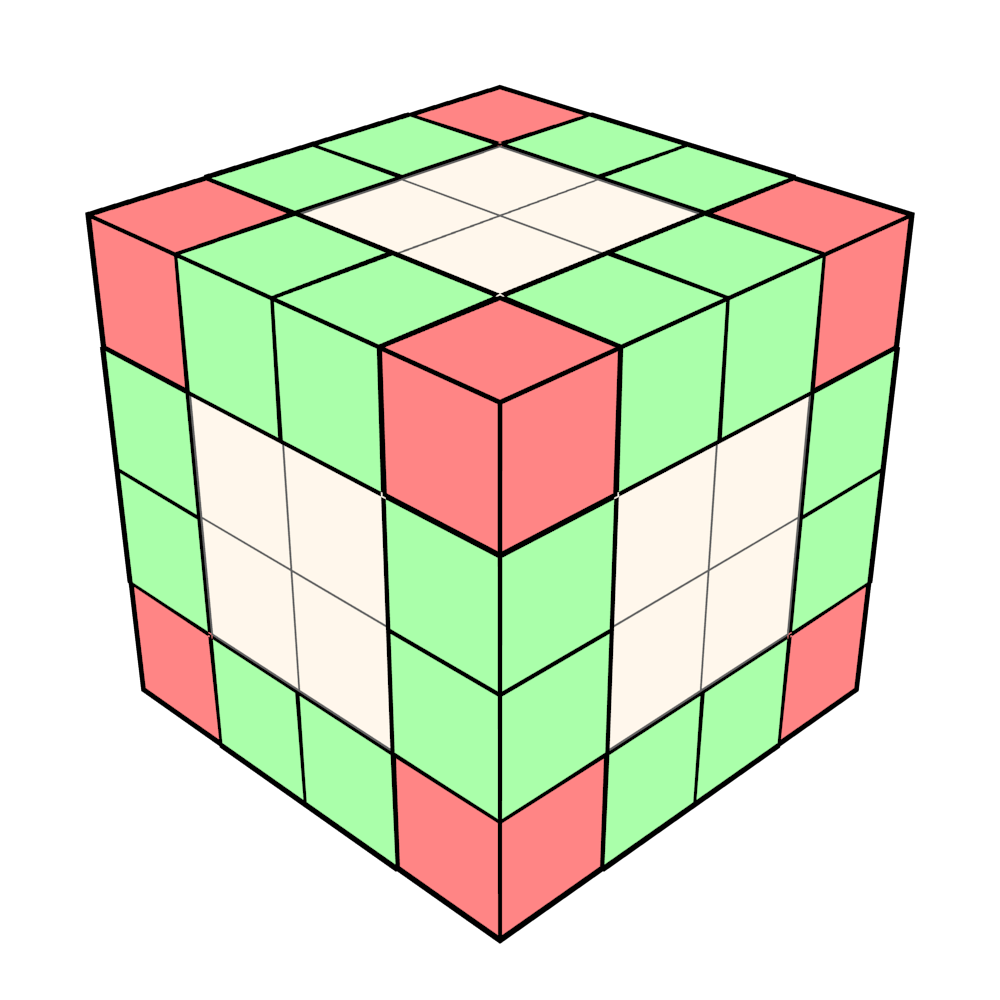
\includegraphics[width=\textwidth]{./img/raw/hs-slt-algorithm/hs-slt-algorithm-8.png}%
    \caption{\footnotesize Mark nodes}%
    \label{fig:hs-p1h}%
  \end{subfigure}
  %
  \begin{subfigure}[b]{.3\linewidth}
    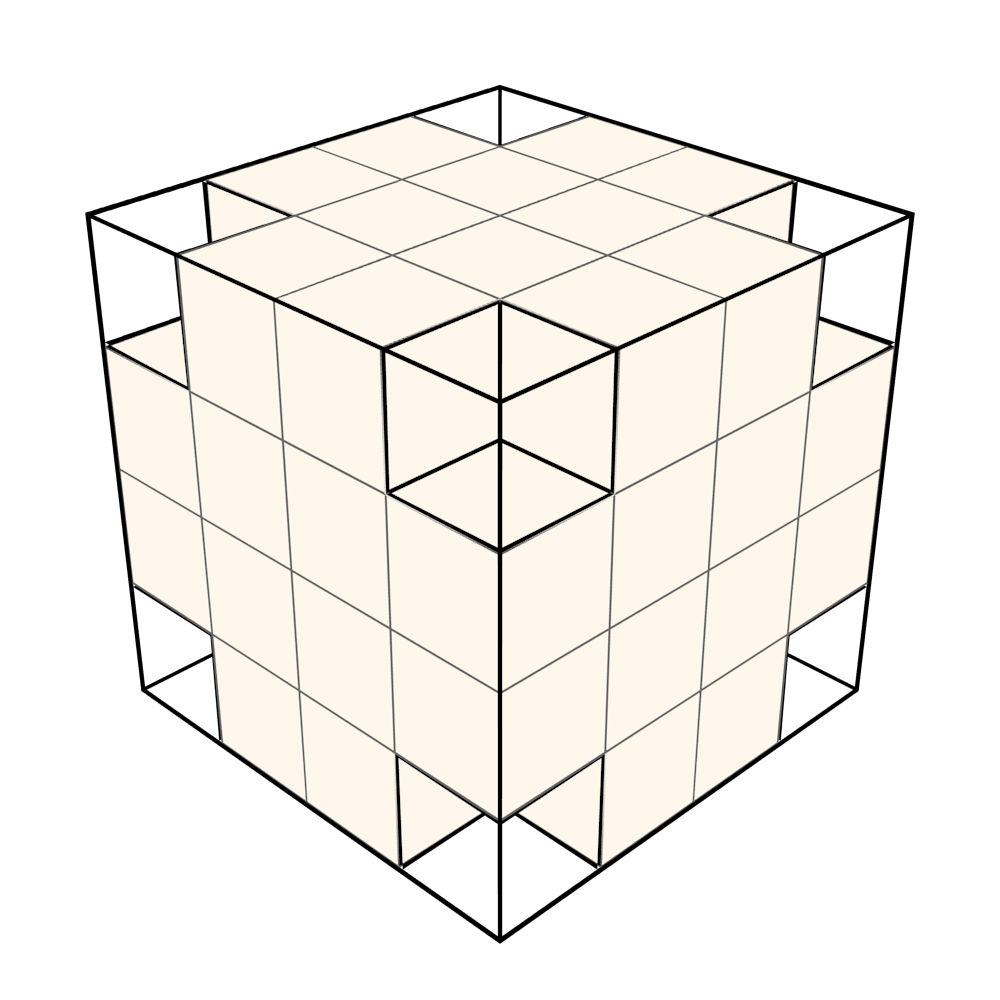
\includegraphics[width=\textwidth]{./img/raw/hs-slt-algorithm/hs-slt-algorithm-9.png}%
    \caption{\footnotesize Finalise grid}%
    \label{fig:hs-p1i}%
  \end{subfigure}

  \caption{Algorithm to determine the overlap of a single light with a grid of minimal nodes.}
  \label{fig:hs-mark}
\end{figure}
